\documentclass[aspectratio=169]{beamer}

\usepackage[T1]{fontenc}
\usepackage[italian]{babel}

\usepackage{hyperref}

\usepackage{tikz}
\usetikzlibrary{positioning, arrows,  decorations.markings}

\title[Pact JVM]{Consumer-driven testing usando Pact JVM}
\institute{Università degli Studi di Milano}
\author[Antonio Tirone]{Antonio Tirone}
\date{2019-2020}

%Qui selezioni tema e colori. http://deic.uab.es/~iblanes/beamer_gallery/
\usetheme{boxes} %Boadilla?
\usecolortheme{seagull}

\tikzset{
 consumer/.style={draw=black, circle, inner sep=0pt, minimum size=2cm
 }
}

\tikzstyle{vecArrow} = [thick, decoration={markings,mark=at position
   1 with {\arrow[semithick]{open triangle 60}}},
   double distance=1.4pt, shorten >= 5.5pt,
   preaction = {decorate},
   postaction = {draw,line width=1.4pt, white,shorten >= 4.5pt}]
\tikzstyle{innerWhite} = [semithick, white,line width=1.4pt, shorten >= 4.5pt]
\begin{document}

\frame{\titlepage}

\begin{frame}
\frametitle{Indice}
\center
\tableofcontents
\end{frame}

\section{Consumer-driven contracts}

\begin{frame}
\frametitle{Consumer-driven contracts}
\begin{itemize}
\item Un pattern per servizi in evoluzione
\item Divenuto uno standard per architetture a microservizi
\item Permette di ridurre al minimo le dipendenze tra componenti diverse
\item Descrivono la comunicazione tra le componenti, non il loro funzionamento
\end{itemize}
\end{frame}
\begin{frame}
\frametitle{Consumer-driven contracts}
\begin{description}
\item[\textbf{Service consumer:}] a component that initiates a HTTP request to another component;
\item[\textbf{Service provider:}] a server that responds to a HTTP request from another component;
\end{description}
Consumer e provider possono essere sviluppati da team o anche da organizzazioni differenti. 
Bisogna assicurare che possano evolvere in maniera indipendente, e non dipendano da una particolare versione dell'altro componente. 
\end{frame}
\begin{frame}[fragile]
\frametitle{Consumer-driven contracts}

\begin{verbatim}
Given "there is no user called Mary"
When "creating a user with username Mary"
  POST /users { "username": "mary", email: "...", ... }
Then Expected Response is 200 OK
\end{verbatim}
\vspace*{1cm}
\begin{verbatim}
Given "there is already a user called Mary"
When "creating a user with username Mary"
  POST /users { "username": "mary", email: "...", ... }
Then Expected Response is 409 Conflict
\end{verbatim}
\end{frame}

\begin{frame}
\frametitle{Consumer-driven contracts}
\center
\begin{tikzpicture}
  \node<1->[consumer](consumer){\textbf{consumer}};
  \node<2->[right = 3cm of consumer](contract){
\includegraphics[width=1.5cm]{./images/contract.png}}; 
  \node<3->[consumer, below= 1.5 cm of contract](provider) {\textbf{provider}};
  \node<4->[left=2.7cm of provider](test){Test Suite};
  
  \draw<2->[->] (consumer) -- node[above]{expectations}(contract);
  \draw<3->[vecArrow, fill] (contract) -- node[right]{communicate} (provider);
%  \draw[innerWhite] (contract) to (provider);
  \draw<4->[->] (provider) -- node[above]{verify}(test);
\end{tikzpicture}
\end{frame}

\begin{frame}
\frametitle{Consumer-driven contracts}
\begin{columns}
  \begin{column}{0.48\textwidth}
Integration test e e2e test:
\begin{itemize}
\item[$+$] confidenza
\item[$-$] introduce dipendenze
\item[$-$] feedback lento
\item[$-$] si rompe facilmente
\item[$-$] richiede molta manutenzione
\end{itemize}
  \end{column}
  \begin{column}{0.48\textwidth}
Contract test:
\begin{itemize}
\item[$+$] confidenza
\item[$+$] eseguiti indipendentemente
\item[$+$] feedback veloce
\item[$+$] stabili
\item[$+$] facili da mantenere
\end{itemize}
  \end{column}
\end{columns}
\vspace*{0.45cm}

Chiaramente i test a contratto non sostituiscono quelli di integrazione, ma possono alleggerirne il carico.
\center
\onslide<2>
NON SONO TEST FUNZIONALI
\end{frame}

\section{Pact}
\begin{frame}
\frametitle{Pact}
\begin{itemize}
\item Consumer-driven contract testing tool
\item Collection of test cases describing single concrete request/response pairs
\item Supports all main languages
\item Communicates through json files
\item Active project
\end{itemize}
\end{frame}

\begin{frame}
\frametitle{Pact}
\center
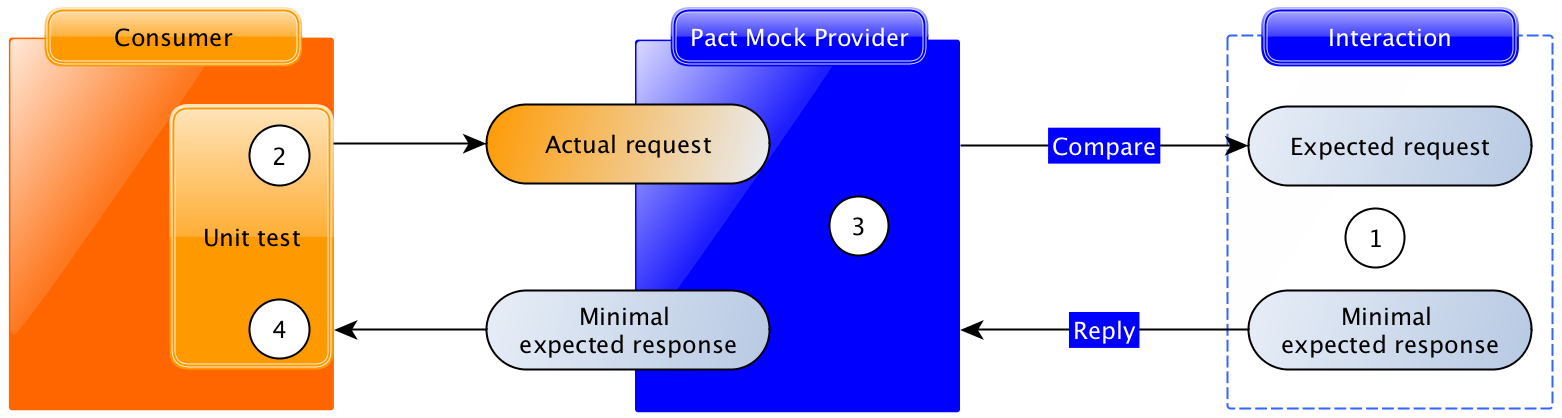
\includegraphics[width=12cm]{./images/pact-overview-consumer.png}
\end{frame}
\begin{frame}
\frametitle{Pact}
\center
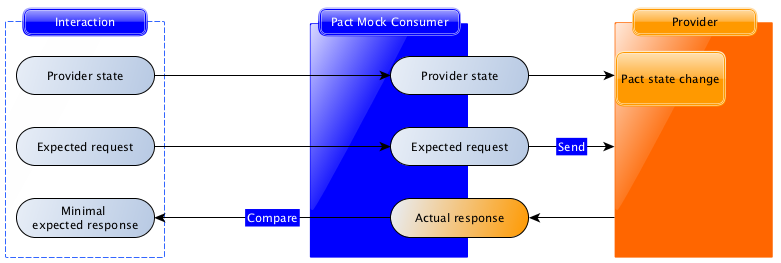
\includegraphics[width=12cm]{./images/pact-verification-states=provider.png}
\end{frame}
\begin{frame}
\frametitle{Pact}
\center
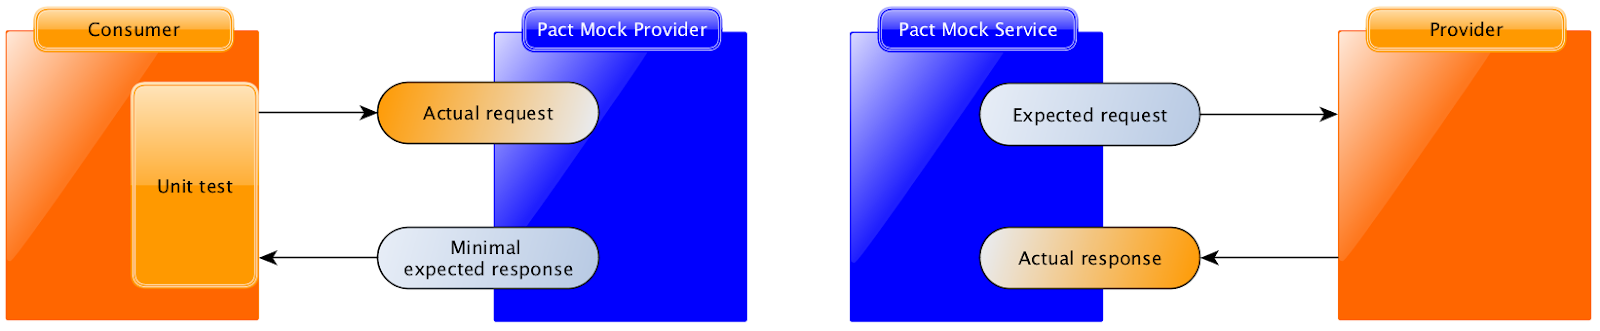
\includegraphics[width=12cm]{./images/pact-test-and-verify.png}
\end{frame}

\section{Pact Broker}
\begin{frame}
\frametitle{Pact broker}
\begin{itemize}
\item Centrale il ruolo della comunicazione
\item Le informazioni su versioni e risultati dei test sono sparse su più build
\item Tool per aggregare i risultati, generando anche documentazione nel processo
\item Supporto per badges

\end{itemize}
\end{frame}
\begin{frame}
\frametitle{Pact Broker}
\center
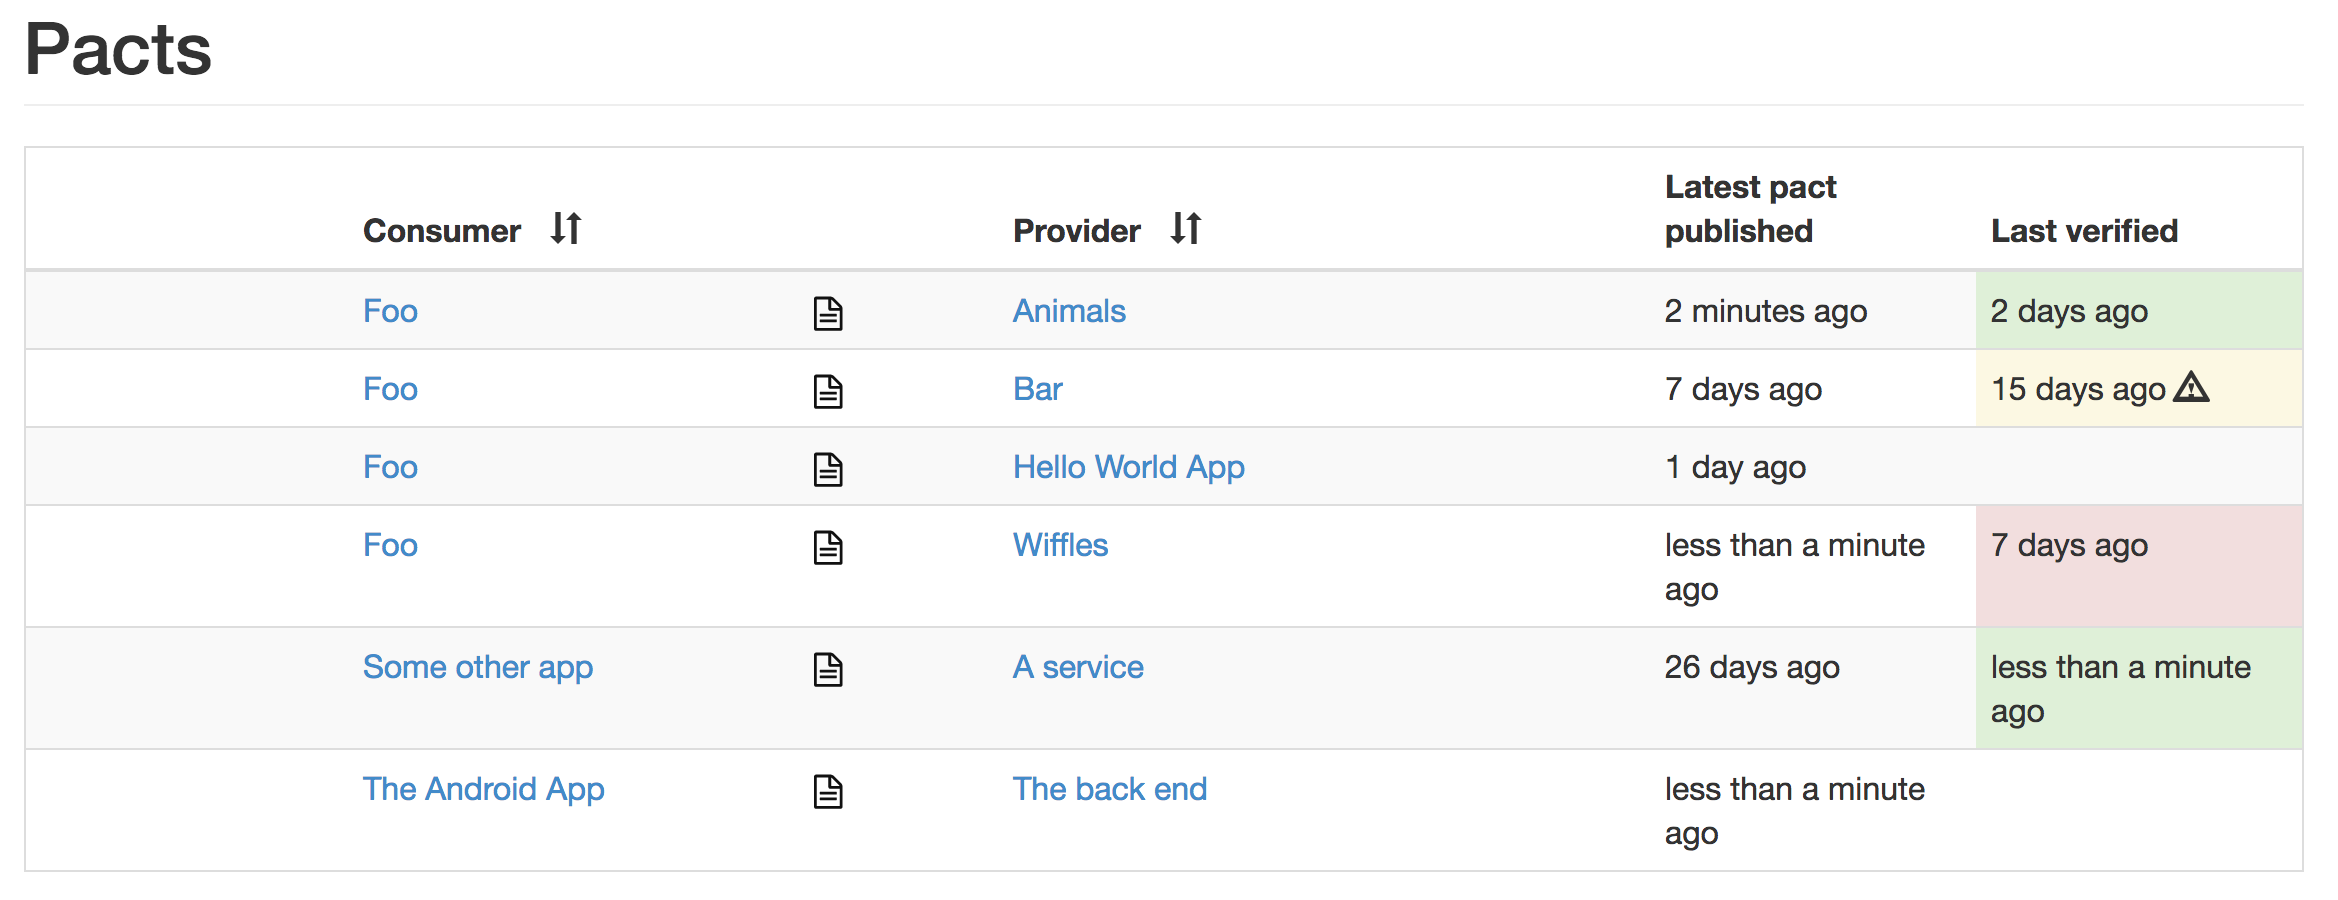
\includegraphics[width=12cm]{./images/pact-broker-index.png}
\end{frame}
\begin{frame}
\frametitle{Pact Broker}
\center
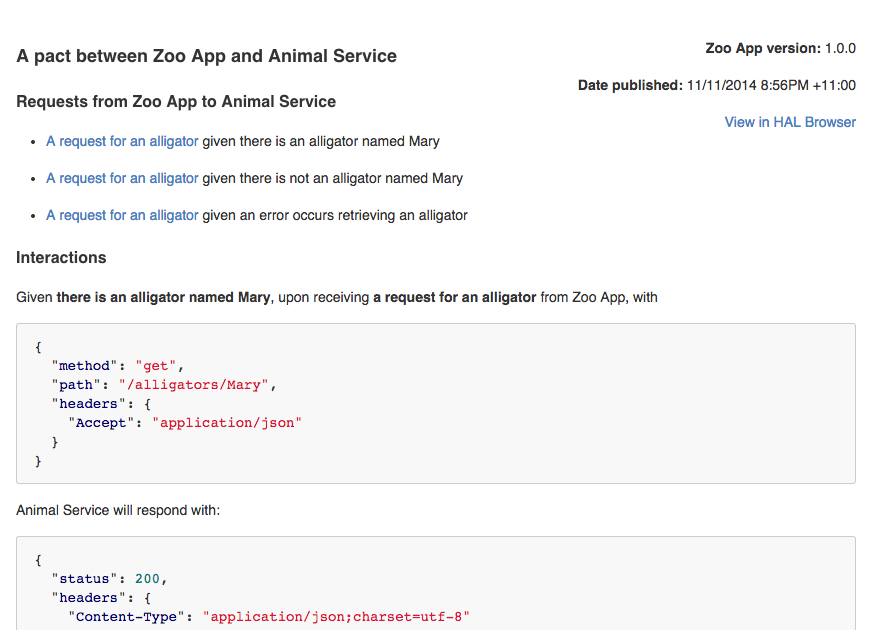
\includegraphics[width=12cm]{./images/autogenerated_documentation.png}
\end{frame}
\begin{frame}
\frametitle{Pact Broker}
\center
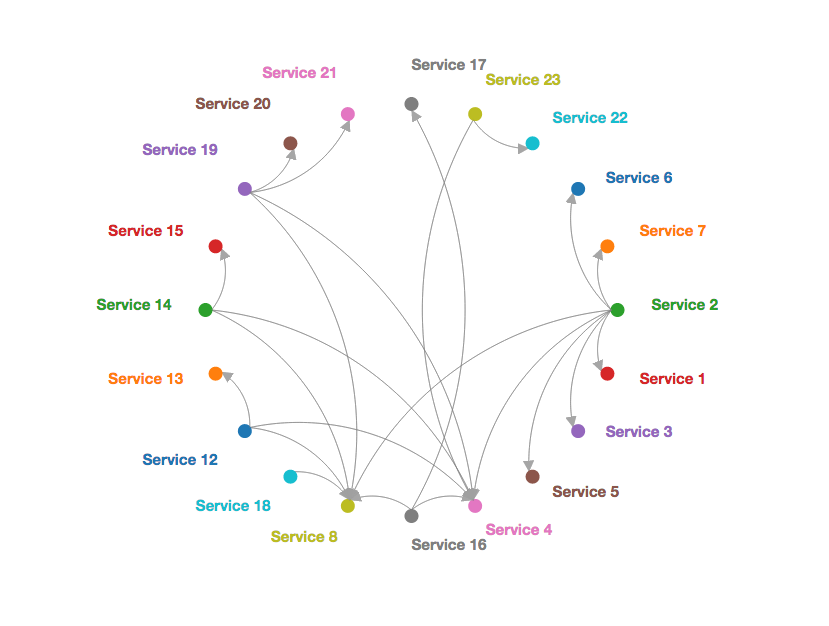
\includegraphics[width=11cm]{./images/network_diagram.png}
\end{frame}

\section{Esempio}
\begin{frame}
\center
\Huge
Esempio
\end{frame}

\begin{frame}
\frametitle{links}

\url{https://martinfowler.com/articles/consumerDrivenContracts.html}

\url{https://github.com/DiUS/pact-jvm/}

\url{https://docs.pact.io/}

\url{https://github.com/pact-foundation/pact_broker}

\url{https://github.com/DiUS/pact-workshop-jvm}

\end{frame}

\end{document}

